\chapter{Implementation}

As we repeatedly mentioned in the first chapter, the design we chose should allow multiple implementations for each module. The implementations provided in this thesis are designed for use-cases ranging from beginner user that requires only core functionality to advanced users who can utilize full module distribution. The resulting implementation therefore offers a monolithic application as well as separate modules.
\par
In this chapter we will discuss the implementation details of every module. At the beginning we will explain our programming language choices. We will add a short description for every library that we used and a reason why we preferred it to others.

%%-----------------------------------------------------------------------------------------
%% SECTION
%%-----------------------------------------------------------------------------------------
\section{Multi-platform Application}

First step on the way to create any piece of software is to select target platform. There are three main platforms, Windows by Microsoft leading the market share with a big margin to OS X by Apple then followed by Linux (see Fig. \ref{fig01:osMarketShareChart}).

\begin{figure}[ht]\centering
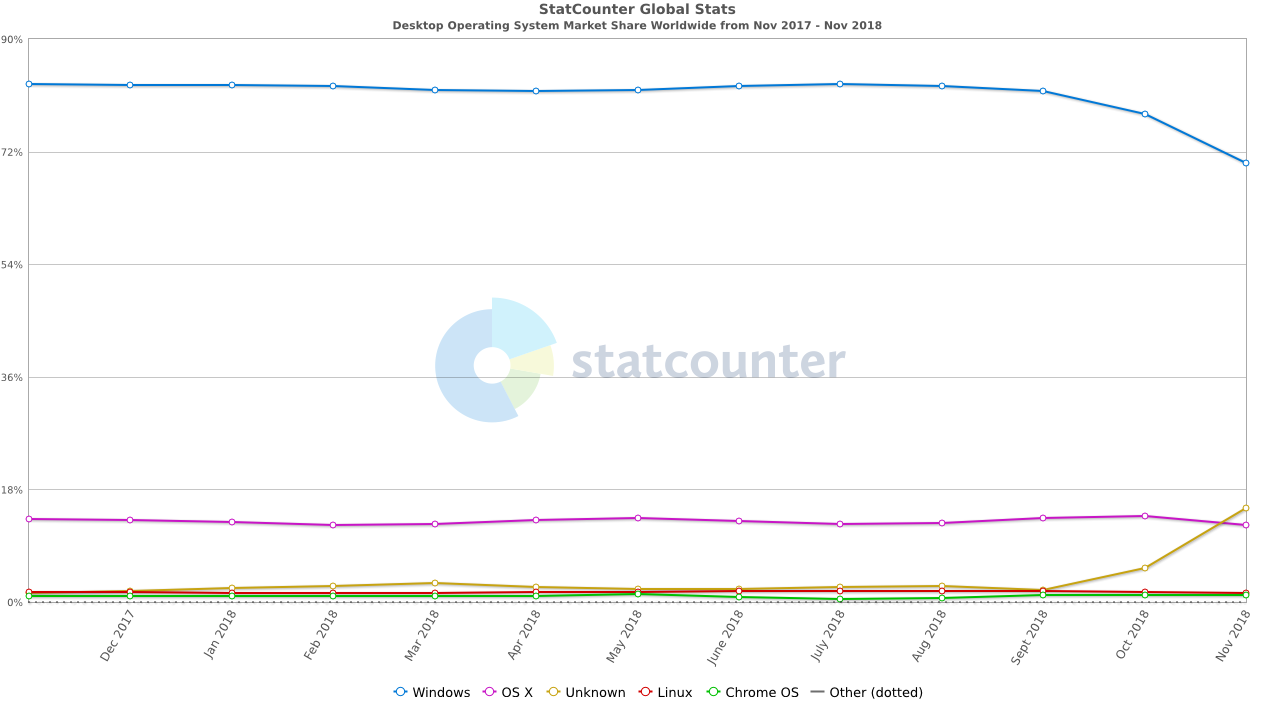
\includegraphics[width=1.0\textwidth]{img/StatCounter-os_combined-ww-monthly-201711-201811}
\caption{Desktop Operating System Market Share Worldwide from Nov 2017 - Nov 2018~\citep{osMarketShare}}
\label{fig01:osMarketShareChart}
\end{figure}

For simplicity we could assume that vast majority of users use Windows and we could target this single platform without losing many potential users. But we do not know the exact market share in our target group and focusing on single platform may be a major mistake.
\par
Another reason to support multiple platforms is the recent progress of miniature PCs. The modular design allows to run each module on a different device and these computers have enough computing power to run Fileserver or Player module that can be separated. They require just a small initial investment into hardware. These PCs usually run or at least support some versions of Linux, which has the smallest market share among major operating systems.
\par
The downside compared to creating platform-specific application is some extra amount of work that needs to be done both during design and implementation. However, we consider the benefits of adopting this approach now to be significant enough compared to the risk of having to support additional platform after the implementation is finished.

%%-----------------------------------------------------------------------------------------
%% SECTION
%%-----------------------------------------------------------------------------------------
\section{Programming Language}

Next decision we had to take was to select a suitable programming language. We had to follow the main guidelines that we have set earlier. That is, we had to find a way to support multiple platforms, while at the same time we needed language flexible enough to handle our modular design.
\par
Even though our modules are separable and therefore each of them could be written in a different language, we wanted to reduce the amount of used languages to minimum, ideally just one or two for the sake of simplicity. Furthermore, we focused on languages that would allow us to write one implementation for all platforms with the minimum of tweaks. Last but not least, we wanted a language that we had at least some experience with.
\par
We have narrowed the choice to three possible main programming languages for our implementation: C++, C\# and Java. All of them are major languages, have cross-platform capabilities and are well-established with enough libraries for all our features. We excluded popular languages Python and JavaScript due to their nature as scripting languages and therefore not providing enough performance for a bigger scale project.

%%-----------------------------------------------------------------------------------------
\subsection{GUI choice}

The weak spot of all three languages is graphical user interface~(GUI) necessary for our Manager module. We would like the GUI to be modern and visually attractive. Common cross-platform GUI frameworks usually either offer a limited set of features, limit customization of them or are difficult to work with. Frameworks for C\#~(WinForms, GTK) and Java~(Swing, JavFX) are good for creating native-looking apps with various forms, but we would like to have more control over graphic design. C++ frameworks have similar issues, the exception might be Qt~\citep{qt}, which is a very capable GUI toolkit written in C/C++, plus there is a Java wrapper for this library available.
\par
We chose the approach with web application wrapped in Chromium Embedded Framework~(CEF). CEF focuses on facilitating embedded browser use cases in third-party applications~\citep{cef}. It means that we can create GUI using HTML5 and JavaScript relying on flexibility, cross-platform support and relative simplicity that they provide compared to other options. CEF offers a way to call C++ code from JavaScript so we can further customize its behavior as a proper desktop application. It is especially useful for I/O calls and operating system interaction.
\par
It is important to note that this decision was influenced by the desire to provide both modular as well as monolithic-looking application. Web GUI can be written once and then be wrapped as desktop application using CEF or slightly modified and utilized as a stand-alone module running on any web browser. Moreover, we can extend it using C++ to bundle it up with the remaining modules and create all-in-one application. Finally, it integrates well with our Data Management module as Firebase provides its SDK in JavaScript.

%%-----------------------------------------------------------------------------------------
\subsection{Final decision}

Having chosen programming languages for Manager module, it remains to choose it for Player and Fileserver modules. Out of the three preselected languages we made C++ our final decision.
Both other languages would be equally capable for the task, but C++ provides more performance and more control of memory management. Furthermore, it does not rely on a virtual machine, which is convenient in case these modules run on a miniature PC, and is already utilized within our Manager module. Lastly, a lot of libraries that work with audio are written directly in C/C++, not always providing a wrapper for Java or C\#.

%%-----------------------------------------------------------------------------------------
%% SECTION
%%-----------------------------------------------------------------------------------------
\section{Manager Module}

Manager module provides user interface for our application. It is written as a single-page web application and runs in an embedded Chromium browser. Other modules are managed from this module by utilising their communication interfaces. Our implementation supports running its own Player and Fileserver module to provide an all-in-one product as well as connecting to remote modules.
\par
The module itself consists of two submodules - web application and browser. As both of them use different programming languages and technologies, different considerations were needed during implementation and so we will describe them separately. At the end, we will sum up how they work together to create this module.

%%-----------------------------------------------------------------------------------------
\subsection{Browser Part}

For the browser part we used Chromium Embedded Framework~(CEF). CEF is a BSD-licensed open source project based on the Google Chromium project. Unlike the Chromium project itself, which focuses mainly on Google Chrome application development, CEF focuses on facilitating embedded browser use cases in third-party applications. It provides close integration between the browser and the host application including support for custom plugins, protocols, JavaScript objects and JavaScript extensions. The host application can optionally control resource loading, navigation, context menus, printing and more, while taking advantage of the same performance and HTML5 technologies available in the Google Chrome Web browser~\citep{cefGithub}.
\par
CEF runs using multiple processes. The main process which handles window creation, painting and network access is called the \textit{browser} process. This is generally the same process as the host application and the majority of the application logic will run in the browser process. DOM rendering and JavaScript execution occur in a separate \textit{render} process~\citep{cefTutorial}. The application behavior can be controlled and modified by overriding callbacks provided by classes of each process. CEF provides default implementation to most of the callbacks.
\par
When the application starts the browser process is created and initialized. Then a new render process is spawned for each unique origin (scheme + domain). In our case there will be a single render process for the web application part. Since CEF runs in multiple processes it is necessary to provide mechanisms for communicating between them~\citep{cefTutorial}. For this CEF provides its own inter-process communication mechanism. Besides exchanging process startup and runtime messages it also supports custom message routing. CEF provides a generic implementation for routing asynchronous messages between JavaScript running in the render process and C++ running in the browser process. The renderer-side router supports generic JavaScript callback registration and execution while the browser-side router supports application-specific logic via one or more application-provided Handler instances~\citep{cefTutorial}. These Handler instances are used to run Fileserver and Player modules within this application instance. They can be started or closed from the web application using registered JavaScript callback.

%%-----------------------------------------------------------------------------------------
\subsection{Web Application Part}

As mentioned earlier, the web application is designed as a single-page web application. The reason to build it that way is simple - usual web pages are served from the server and running a server for this purpose would make little sense. Single-page applications~(SPA) are loaded once at the beginning~(HTML, JavaScript and CSS code) and instead of loading new pages from server they dynamically rebuild the current page. These applications have become popular recently and provide a solution to some problems web applications have compared to traditional web page design. Namely, stateless nature of web pages and wait time due to loading. On the other hand, SPA brought their own problems but most of them can be solved by some useful JavaScript libraries, packages and frameworks. One of the main negatives - speed of initial load when all required code is loaded at once is irrelevant for us. It is all stored locally on the device. Compared to the speed of network data transfers it is negligible.

%%-----------------------------------------------------------------------------------------
\subsubsection{GUI Design}

The GUI is divided into multiple boards that the user can switch between using navigation bar at the top of the screen. Each board offers controls for different tasks. At the bottom of the screen is player bar offering access to player controls across all boards. There are 5 boards:
\begin{itemize}
    \item Library
    \item Establishment
    \item Playback
    \item Devices
    \item Settings
\end{itemize}
\par
Library board displays contents of the music library of connected Fileserver module. It offers controls for filtering available songs, browsing genres, albums and artists and creating and modifying playlists defined by the spot admin. Any list of songs in the library can then be selected for music playback. If the application uses local Fileserver, it also provides controls for adding and removing music files in the library.
\par
Establishment board displays general information about the music spot that guests can see in mobile application.
\par
Playback board is used to manage music playback. It displays list of currently available songs and details of queues. There are three available queues: priority, order and playlist queue. Priority queue can be used by spot admin to select songs to play with highest priority. Order queue is filled with songs ordered by guests. Playlist queue contains songs that will play when there are no songs in other two queues. Songs generated by Manager module are added to this queue.
\par
Devices board is used to manage connections to Fileserver and Player modules. Users may choose to use a local module launched by this application or connect to a remote module.
\par
Settings board is used for editing application settings.

%%-----------------------------------------------------------------------------------------
\subsubsection{Framework}

There are a few frameworks for building single-page applications. They all provide their way of rebuilding the page and data management. Most of them are labeled as MVC frameworks. It is important to note that we chose our framework early in 2017 and since then a lot has changed. We were effectively choosing between Angular.JS and React.JS. The rest of the frameworks did not have large enough community or support at that time so we did not take them into consideration.
\par
To be precise, React is not labeled as framework but as a JavaScript library. Its role is to make creating interactive user interfaces easier. It has to be coupled with Redux, a predictable state container for JavaScript apps to reach the capabilities of Angular. In this form, we think both Angular and React + Redux can be used to do the same work, it is just a matter of personal choice and preference.
\par
It is difficult to write a comparison between React and Angular as they release new features on frequent and regular basis. Many up-to-date articles comparing them and also other new frameworks such as Vue.js can be found online. Here is a list of arguments that we took into consideration:
\begin{itemize}
    \item Angular is a complete framework that provides more features out of the box compared to React, which has to supply them using various community-provided packages
    \item Angular more strictly enforces the way the applications should be build which makes it more difficult to learn it initially
    \item React is considered to be faster based on various benchmarks due to its refined \textit{Virtual DOM} rendering mechanism
    \item We consider React JSX syntax allowing HTML markup and JavaScript code to be merged in a single file to be a good tool for increasing productivity
    \item React has wider community of developers and supporters
\end{itemize}
\par
We chose to use React + Redux as our framework for web application. We find the syntax and concept more natural and simple to use as we had no previous experience with either of them. The performance advantage is also important as Manager module needs to handle more tasks than just rendering the GUI. It is important to mention again that Angular would be equally capable for the job, we just value React more. Also, at the time we made the choice, Angular 2 was released that introduced multiple improvements in favor of Angular, but it was too new at the time.

%%-----------------------------------------------------------------------------------------
\subsubsection{Design Principles}

JavaScript is more forgiving compared to strong-typed compiled object-oriented programming languages so good code structure is important to maintain readability of code. Application design therefore follows recommended React and Redux design principles. The code becomes structured and is split into several types of code files. Every type contains specific functionality and extracts it from the others so similar functionality is grouped together. Below is the list of code file types and their description.

\begin{itemize}
    \item \textbf{Components} contain layout of the page – they display data supplied to it and link supplied actions to layout elements. They are usually stateless. There are two types of components, layout components that represent a whole page and visual components that represent a reusable functional element within a page
    \item \textbf{Containers} contain functionality and business logic – functions, event callbacks, state management and data preparation methods passed to components. They encapsulate components, therefore they are called containers. 
    \item Redux \textbf{store} is used to preserve shared state of the application.
    \item \textbf{Reducers} react to actions and change the data stored in the store.
    \item \textbf{Actions} trigger changes on the store. For every reducer there is a set of actions and action creators. Every action creator may create zero, one or more actions depending on the conditions.
\end{itemize}

\begin{figure}[ht]\centering
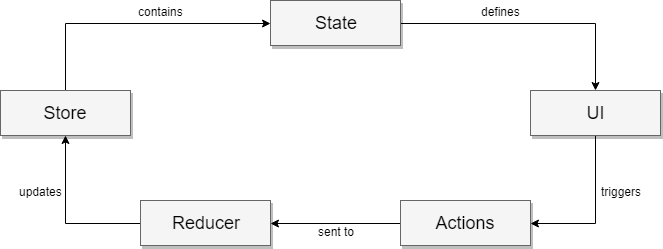
\includegraphics[width=1.0\textwidth]{img/reactReduxFlow.png}
\caption{React + Redux flow}
\label{fig04:reduxFlow}
\end{figure}

The flow of React + Redux application can be seen in figure \ref{fig04:reduxFlow}.
\par
Similarly to common web pages the page layout is determined by path, in React called "route". However, the route is only symbolic as the page remains the same. Navigating to different routes forces application to re-render it's content. Nesting the route can make only a part of the page to re-render.
\par
The layout is determined by the state stored in store. Before the rendering begins the state is applied to all component and the resulting layout is rendered.
\par
When an event occurs on a component, an action is triggered. Actions can range in complexity from a simple state property change to triggering multiple other actions, making AJAX request and others. Actions can send state change requests to reducers.
\par
Reducers are the only place where store state can be changed. They process state change requests and return a new state object. State objects are always immutable. A store consists of multiple state objects and every state object is handled by its reducer. State change triggers current page to re-render, providing it with the new state and the loop completes.

%%-----------------------------------------------------------------------------------------
\subsubsection{Communication With Other Modules}

To communicate with Fileserver module, we use axios library. It is an asynchronous HTTP client for the browser and node.js~\citep{axios}. We use it to send asynchronous HTTP requests to Fileserver. It simplifies sending AJAX requests and provides modern Promise API. 
\par
WebSocket communication with Player module utilizes default WebSocket object that provides JavaScript. Upon establishing connection with Player, the created socket is stored in state. Actions that send messages to Player access this instance to do so. A callback function is provided to the constructor that handles incoming messages. Incoming messages are processed and corresponding action is triggered.
\par
Firebase provides software development kit~(SDK) in JavaScript. Every communication with Data Management module utilizes this SDK. It provides methods for reading and manipulation of data as well as hook up callbacks. When the user signs in, an authentication token is received and all subsequent calls to firebase use this authentication. Module initially loads music spot information. When spot admin selects a list of songs for playback, these are processed to match firebase structure, uploaded and it subscribes to queue change notifications. When the playback ends, list of songs and queue are removed to clean up the database.

\subsubsection{JavaScript Libraries Used}

We used multiple packages and libraries from Node.js Packet Manager~(NPM). We will mention important ones.
\par
Material-UI library offers styled React components in popular material design developed by Google. We used these components to create a modern and appealing UI which should look familiar to users.
\par
React-intl library is used to create a localized application. All strings in components are grouped in "messages.js" file next the files containing layout, marked with unique identifier and a default translation is supplied. When a string is needed its identifier is passed to a function from react-intl library which takes care of finding the right translation. When the application is built all strings are extracted to a JSON file. Multiple JSON files can be provided with different translations to support multiple languages.
\par
React-virtualised library provides infinite and virtual scroll components. The data in music library are loaded in small amounts using AJAX requests. Infinite scroll allows to dynamically load more data when they need to be displayed to user. Virtual scroll is necessary to deal with displaying long lists of data. With growing number of items in a list, more DOM elements are required to render the it. The more DOM elements the rendering becomes slower and slower. Virtual scroll renders only a few items that the user can see on screen and dynamically changes contents of these elements as the user scrolls.

%%-----------------------------------------------------------------------------------------
\subsection{Bringing The Module Together}

On module startup the browser is run and initialized. When it is ready the web application is loaded from local storage. The application is displayed and users can work with it. The web application utilizes message router provided by CEF to communicate with browser using . We registered a callback function \texttt{cefQuery} in JavaScript that allows sending messages to browser code. After users log in local Fileserver and Player are started utilising \texttt{cefQuery} function and connected to. These can be shut down and users may connect to other modules from "Devices" menu. 

%%-----------------------------------------------------------------------------------------
%% SECTION
%%-----------------------------------------------------------------------------------------
\section{Fileserver Module}

This implementation of Fileserver module allows creating private music databases on computers and devices of spot admins. It consists of two main parts - data storage for music file metadata and HTTP API.

%\subsection{Libraries Used}
%We used two third-party libraries for the implementation of this module.
%\par
%First one is SQLite that we used for data storage. SQLite is a C-language library that implements a small, fast, self-contained, high-reliability, full-featured, SQL database engine. SQLite is the most used database engine in the world. SQLite is built into all mobile phones and most computers and comes bundled inside countless other applications that people use every day. The SQLite file format is stable, cross-platform, and backwards compatible and the developers pledge to keep it that way through at least the year 2050. SQLite database files are commonly used as containers to transfer rich content between systems and as a long-term archival format for data. There are over 1 trillion SQLite databases in active use~\citep{sqlite}. It allows us to to create a small SQL database file locally on the device where it runs.
%\par
%The other library we used is called C++ REST SDK~(cpprestsdk). The C++ REST SDK is a Microsoft project for cloud-based client-server communication in native code using a modern asynchronous C++ API design. This project aims to help C++ developers connect to and interact with services. Microsoft have developed this library, because historically C++ developers have been lacking a basic set of tools that enable them to access and author REST services in a productive, scalable and asynchronous manner. C++ Rest SDK aims to alleviate some of the pain felt by developers by providing a cross-platform library that is modeled on simplicity, extensibility and composition~\citep{cpprestsdk}. Even though C++ is not a preferred language for creating REST services, this library offers a simple way for both creating and accessing these services. It handles the network communication for us and allows us to focus on the business logic that processes and delivers data.
%\todo{maybe add that their are open source and cross platform? mention troubles with cpprestsdk?}

%%-----------------------------------------------------------------------------------------
\subsection{Data Storage}

Data storage is required to store music file metadata of music library. Extracting metadata takes time as sometimes whole files have to be scanned, so storing once extracted metadata increases performance. 
\par
We also want to store location of these music files. They can be located anywhere in a file system of the used device. Storing the location allows spot admins to preserve their preferred file structure, they just need to specify which files they want to include in music library.
\par
Data storage then needs to support certain operations required by HTTP API. The API requires the ability to effectively search different attributes of song metadata. A common approach to enable data queries would be to store it in a relational database to make use of the power of SQL. Most relational database management systems~(RDBMS) require a server to access the database. It is inconvenient to set up such server in target use cases of this module. Instead, we used SQLite library that implements a self-contained, server-less, zero-configuration SQL database engine~\citep{sqlite}. It can easily store thousands of records, which is sufficient.
\par
The database schema can be seen in figure \ref{fig03:dbSchema}.
\begin{figure}[ht]\centering
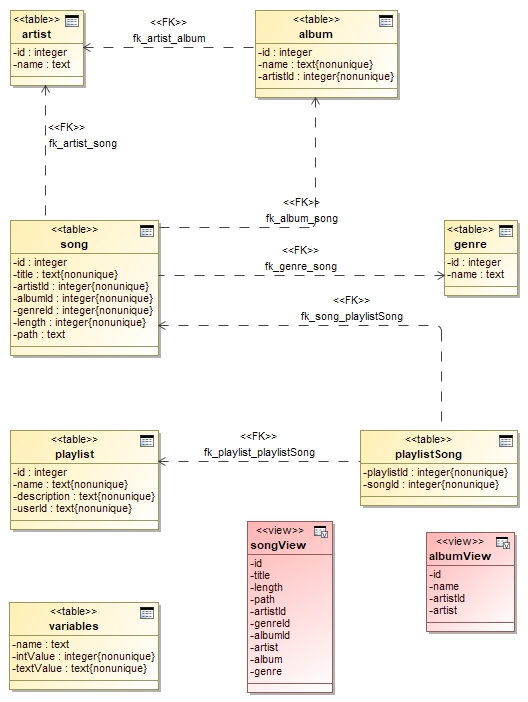
\includegraphics[width=1.0\textwidth]{img/DbDiagram2.png}
\caption{Database schema}
\label{fig03:dbSchema}
\end{figure}
\par
We implemented a single class that takes care of working with the database named \texttt{SqliteAPI}, as it provides an API for working with our SQLite library. This class executes SQL queries and returns data from database. Methods that retrieve data accept a list of parameters that allow filtering and modifying results of their query.
This class also offers methods for adding and removing songs into/from music library.
\par
\texttt{AudioInspector} class implements extraction of metadata from music files using ffmpeg library \citep{ffmpeg}.

%%-----------------------------------------------------------------------------------------
\subsection{HTTP API}
% vediet prijat http request
% spracovat
% ziskat data z DB
% transformovat do JSON
% poslat naspat

We need to be able to handle HTTP requests. This includes:
\begin{enumerate}
    \item Receiving HTTP requests
    \item Processing incoming requests
    \item Retrieving data from data storage
    \item Transformation of data into JSON format
    \item Returning response with data
\end{enumerate}

In order to receive and send HTTP requests we used C++ REST SDK library~\citep{cpprestsdk}. It provides an HTTP listener that listens for incoming requests and a set of asynchronous methods to handle these requests in a modern and efficient way. It provides its own implementation of asynchronous tasks.
\par
To create an abstraction between the HTTP listener and data storage we utilized the bridge design pattern. It allowed us to create HTTP listener independent from data storage. Coupling it with another data storage would just require implementing the abstract class \texttt{AbstractFileServerHandler} in a new bridge.
\par
The \texttt{FileServerAPI} class wraps the HTTP listener. Upon receiving a request from HTTP listener a corresponding HTTP method handler parses URI and parameters and validates the request. Then it passes the parameters to a corresponding method of the associated bridge which executes the action and returns data for the response. This response is then sent back to the client.
\par
\texttt{FileServerHandler} class is a bridge implementation for SQLite data storage. It owns an \texttt{SqliteAPI} class instance and calls its methods to retrieve data for requests. It then transforms the data to JSON format supported by HTTP API.
%It supports \texttt{GET}, \texttt{POST}, \texttt{PUT} and \texttt{DELETE} request methods required by HTTP API design and adds \texttt{OPTIONS} method to provide cross-origin resource sharing~(CORS) headers. These are important to support Manager module running on a browser that restricts cross-origin HTTP requests to access this API.

%%-----------------------------------------------------------------------------------------
%% SECTION
%%-----------------------------------------------------------------------------------------
\section{Player Module}

The main feature of Player module is playing music. Besides that, it is important to implement caching functionality and API for communication over WebSocket.

%%-----------------------------------------------------------------------------------------
%\subsection{Libraries Used}
%We utilized three third-party libraries in this module. Two are used for audio playback and one for communication interface.
%\par
%FFmpeg is the leading multimedia framework, able to decode, encode, transcode, mux, demux, stream, filter and play pretty much anything that humans and machines have created. It supports the most obscure ancient formats up to the cutting edge. No matter if they were designed by some standards committee, the community or a corporation. It is also highly portable: FFmpeg compiles, runs, and passes testing infrastructure FATE across Linux, Mac OS X, Microsoft Windows, the BSDs, Solaris, etc. under a wide variety of build environments, machine architectures, and configurations~\citep{ffmpeg}. Basically, this library allows us to support any music file format we  would like to. We utilised it in Fileserver module for metadata extraction, but it is utilised more heavily here for audio decoding.
%\par
%To output decoded audio to speakers, we used PortAudio library. PortAudio is a free, cross-platform, open-source, audio I/O library. It lets you write simple audio programs in 'C' or C++ that will compile and run on many platforms including Windows, Macintosh OS X, and Unix (OSS/ALSA). It is intended to promote the exchange of audio software between developers on different platforms. Many applications use PortAudio for Audio I/O~\citep{portaudio}. This library offers cross-platform access to audio I/O as all platforms have their own way of working with it.
%\par
%Even though C++ REST SDK that we used in Fileserver module promises WebSocket functionality, it only supported WebSocket client at the time. We need to build a WebSocket server so we had to choose different library. For this task we chose Boost.Beast library. Beast is a C++ header-only library serving as a foundation for writing interoperable networking libraries by providing low-level HTTP/1, WebSocket, and networking protocol vocabulary types and algorithms using the consistent asynchronous model of Boost.Asio~\citep{beast}. While this library provides low-level tools, we needed to build just a small server so it allowed us to customize it to create simple and small implementation with the benefits of asynchronous programming from Boost.Asio library.
%\todo{write about boost, ffmpeg and portaudio}

%%-----------------------------------------------------------------------------------------
\subsection{File Caching}

We need to download and cache music files in advance to have them ready for playback. 
\par
Cached files can be stored in storage or in memory. This decision is important for miniature PCs that operate with limited resources. Storage option would allow us to cache more songs and provide larger cache for big files. However, these devices usually use flash drives for storage which do not handle frequent writes very well and usage of our application would wear these memories down too early.
\par
Storing cached music files in memory is limited by memory capacity which is usually between 1 and 4 GB on these devices. To provide a smooth music playback we would like to have at least three songs cached - one being played, one ready to be played next and one being loaded. An average size of a music file using compressed format can be around 10MB, so three files would take up 30 MB of space. This should not cause any problems. Even using lossless file formats where file sizes are around 70MB would require just 210MB which should be possible to handle.
\par
We decided to store cached files in memory. To provide a little more robustness we always try to cache 3 songs and one additional song is being played. In case there are less than 3 songs provided by Manager module, this implementation notifies it using API notification to supply more songs until the cache is full.
\par
Caching is implemented in \texttt{SongCache} class. This class contains HTTP client from C++ REST SDK library that it uses to download music files into cache. On input it receives queue of songs and outputs next music file to be played.
%\par
%Internally, \texttt{SongCache} utilizes \texttt{SongCacheItem} class for storing each queued item. This class holds an asynchronous buffer that is used to download the data asynchronously and upon completion it provides a \texttt{std::basic\_istream} for reading cached file contents. Before accessing it, it is necessary to check for errors.

%%-----------------------------------------------------------------------------------------

\subsection{Audio Decoding and Playback}

Playing audio files is done in two steps. First, music file has to be decoded to produce pulse-code modulation~(PCM) data which are then sent to the output audio device.
We utilize ffmpeg library~\citep{ffmpeg} for audio decoding and PortAudio library~\citep{portaudio} for working with audio device. When audio device needs data for playback, PortAudio asynchronous callback function is run. Within this function required amount of music samples are decoded using ffmpeg library and written to buffer of audio device. This functionality is contained within \texttt{MusicPlayer} class.
%\par
%Before the playback can start, it is necessary to call \texttt{Open} method. This method prepares the music file for playback. The process consists of these steps:
%\begin{itemize}
%    \item Creating custom \texttt{AVIOContext} that supports reading data from \texttt{std::basic\_istream} by providing read and seek function and a buffer for data
%    \item Opening the file and finding stream information
%    \item Using stream information to detect audio stream within the file and finding appropriate decoder for the stream format
%    \item Initializing selected decoder 
%    \item Initializing audio output device to correctly interpret data provided by audio stream and decoder
%    \item Initializing PortAudio output stream and providing it with the \texttt{StreamInfo} structure that we filled in previous steps
%\end{itemize}

%%-----------------------------------------------------------------------------------------
\subsection{WebSocket API}

This module implements a WebSocket server that awaits connection from a Manager module. We used Boost Beast library~\citep{beast} that takes care of asynchronous communication over WebSocket.
\par
The functionality of the server is layered into multiple classes. At the top is the \texttt{API} class. This class wraps the entire server and offers methods to start and stop the server.
\par
When the server is started, \texttt{API} class instance runs an instance of \texttt{Listener} class. This class provides functionality to listen for and accept incoming connections asynchronously.
\par
After a new connection is accepted, an instance of \texttt{Session} class takes over the created socket and handles the incoming ant outgoing communication. It represents a session of Player module during which the music playback occurs. This instance owns song cache and music player and takes care of cooperation between them. Reads and writes on WebSocket are performed asynchronously. 

%%-----------------------------------------------------------------------------------------
%% SECTION
%%-----------------------------------------------------------------------------------------
\section{Data Management Module}

Data Management module utilizes firebase platform. It uses its Authentication feature and Realtime Database.
\par
Authentication feature is used to authenticate users. They can use e-mail and password to sign in. Authentication tool manages registered users and safely stores their passwords and provides authentication tokens to signed in users. This token is required to access Realtime Database.
\par
Realtime Database stores data that are exchaged between spot admins and guests. This is a NoSQL database in JSON format. Applications can access this database using Firebase SDK. It provides a set of functions for data manipulation. To read or modify the data, application has to specify which node within the JSON structure it is interested in. These functions are then applied to this node.
\par
In Realtime Database, clients implement logic for working with it. Realtime Database is schemaless, so it is important to ensure data consistency since data manipulation is distributed among clients. It supports defining a set of rules to validate consistency of database structure and to restrict access to data. Validation rules ensure that writes preserve consistent structure. Authorization rules restrict read and write access to database. Authorization rules cascade, so granting read/write access to a node grants same access to nodes nested under it~\citep{firebaseDocs}.

\paragraph{Database Structure}
\begin{code}
libraries : [spotId] : Library
que : [spotId] : QueItem
spots : public : [spotId] : PublicSpotInfo
      : private : [spotId] : PrivateSpotInfo
users : public : [userId] : PublicUserInfo
      : private : [userId] : PrivateUserInfo
\end{code}


\paragraph{Entities Structure}
\begin{code}
PublicUserInfo : [userId]
    name : String

PrivateUserInfo : [userId]
    credits : Number @Optional
    adminForSpot : [spotId] @Optional

QueItem : [pushId]
    songId : String
    userId : String @Optional # if missing then item was added by spot
    
PublicSpotInfo : [spotId] 
    name : String
    active : Boolean
    description : String
    address : String

PrivateSpotInfo: [spotId]
    billingInfo : BillingInfo

BillingInfo
    bankAccount : String
    variableSymbol : String
    
Library : [spotId]
    artists : [artistId] : MusicEntity
    albums : [albumId] : MusicEntity
    genres : [genreId] : MusicEntity
    songs : [songId] : Song
    lists : [songListId] : List
    
List : [songListId]
    [songId] : Boolean # always true
    
MusicEntity : [id]
    songListId : [songListId]
    name : String

Song : [songId]
    name : String
    length : Number
\end{code}